\section*{Assignment 07: Inequality and Responsibility}
\addcontentsline{toc}{section}{Assignment 07: Inequality and Responsibility}

\subsection*{Diagnosing inequality risks}
I used Lecture~8’s inequality checklist \citep{Lecture08}. Resource light NGOs worry about hidden costs and have too few staff to run another platform. Humanities and design faculties often find their work pushed aside because evaluation focuses on business results. \citet{Srnicek2017} and \citet{Choudary2016} both explain that governance must fit the \textit{participant value logic}, otherwise \textit{network effects} increase inequity. These insights guide the planned interventions.

\subsection*{Targeted interventions with evidence}
\begin{itemize}
  \item \textbf{Resource light NGOs.} I package a lean onboarding kit: templated briefs, an auto generated progress report, and a buddy system where experienced students shadow the first sprint. The VirtuAI case showed how social onboarding offsets scarce staff, so this kit directly applies that lesson \citep{Gunasilan2024}.
  \item \textbf{Humanities and design faculties.} Faculty sandboxes let departments define success metrics beyond revenue, including qualitative reflection and cultural impact. The sandbox also supports offline uploads for analogue prototypes. This follows \citet{Reillier2017}'s guidance on modular governance so each segment keeps legitimacy.
  \item \textbf{Cross campus community.} A fairness clause tracks hours contributed versus fees paid and unlocks waivers once volunteer time passes a threshold. An inclusion council with representatives from every faculty and NGO cluster reviews data policy changes quarterly. Finally, an impact audit inspired by the DineTogether case checks whether new features skew toward well funded actors \citep{Rennella2023}.
\end{itemize}

\subsection*{Operationalising fairness}
To put these ideas into practice I created concrete artefacts. The onboarding kit is stored in a shared Notion space with checklists, video walkthroughs and a budget calculator. Faculty sandboxes start as private workspaces filled with templates for qualitative assessment. The \textit{fairness clause} is placed inside the terms of use with a clear rule: if an organisation contributes more than thirty unpaid hours in a quarter, its transaction fees are reduced by half for the next two briefs. \textit{Inclusion council} meetings follow an agenda inspired by \citet{Lecture11}'s discussion of legitimacy: review metrics, approve policy changes and hear community concerns.

The messaging system in Figure~\ref{fig:chat-system} connects all parts. Dedicated channels handle \textit{accessibility requests}, \textit{translation help}, and \textit{fairness feedback}. Moderators use prepared replies that link to the related clause so tone stays consistent while keeping empathy. This setup treats communication as part of the core structure, following \citet{Choudary2016}'s advice to support \textit{community level interactions}.

\begin{figure}[H]
  \centering
  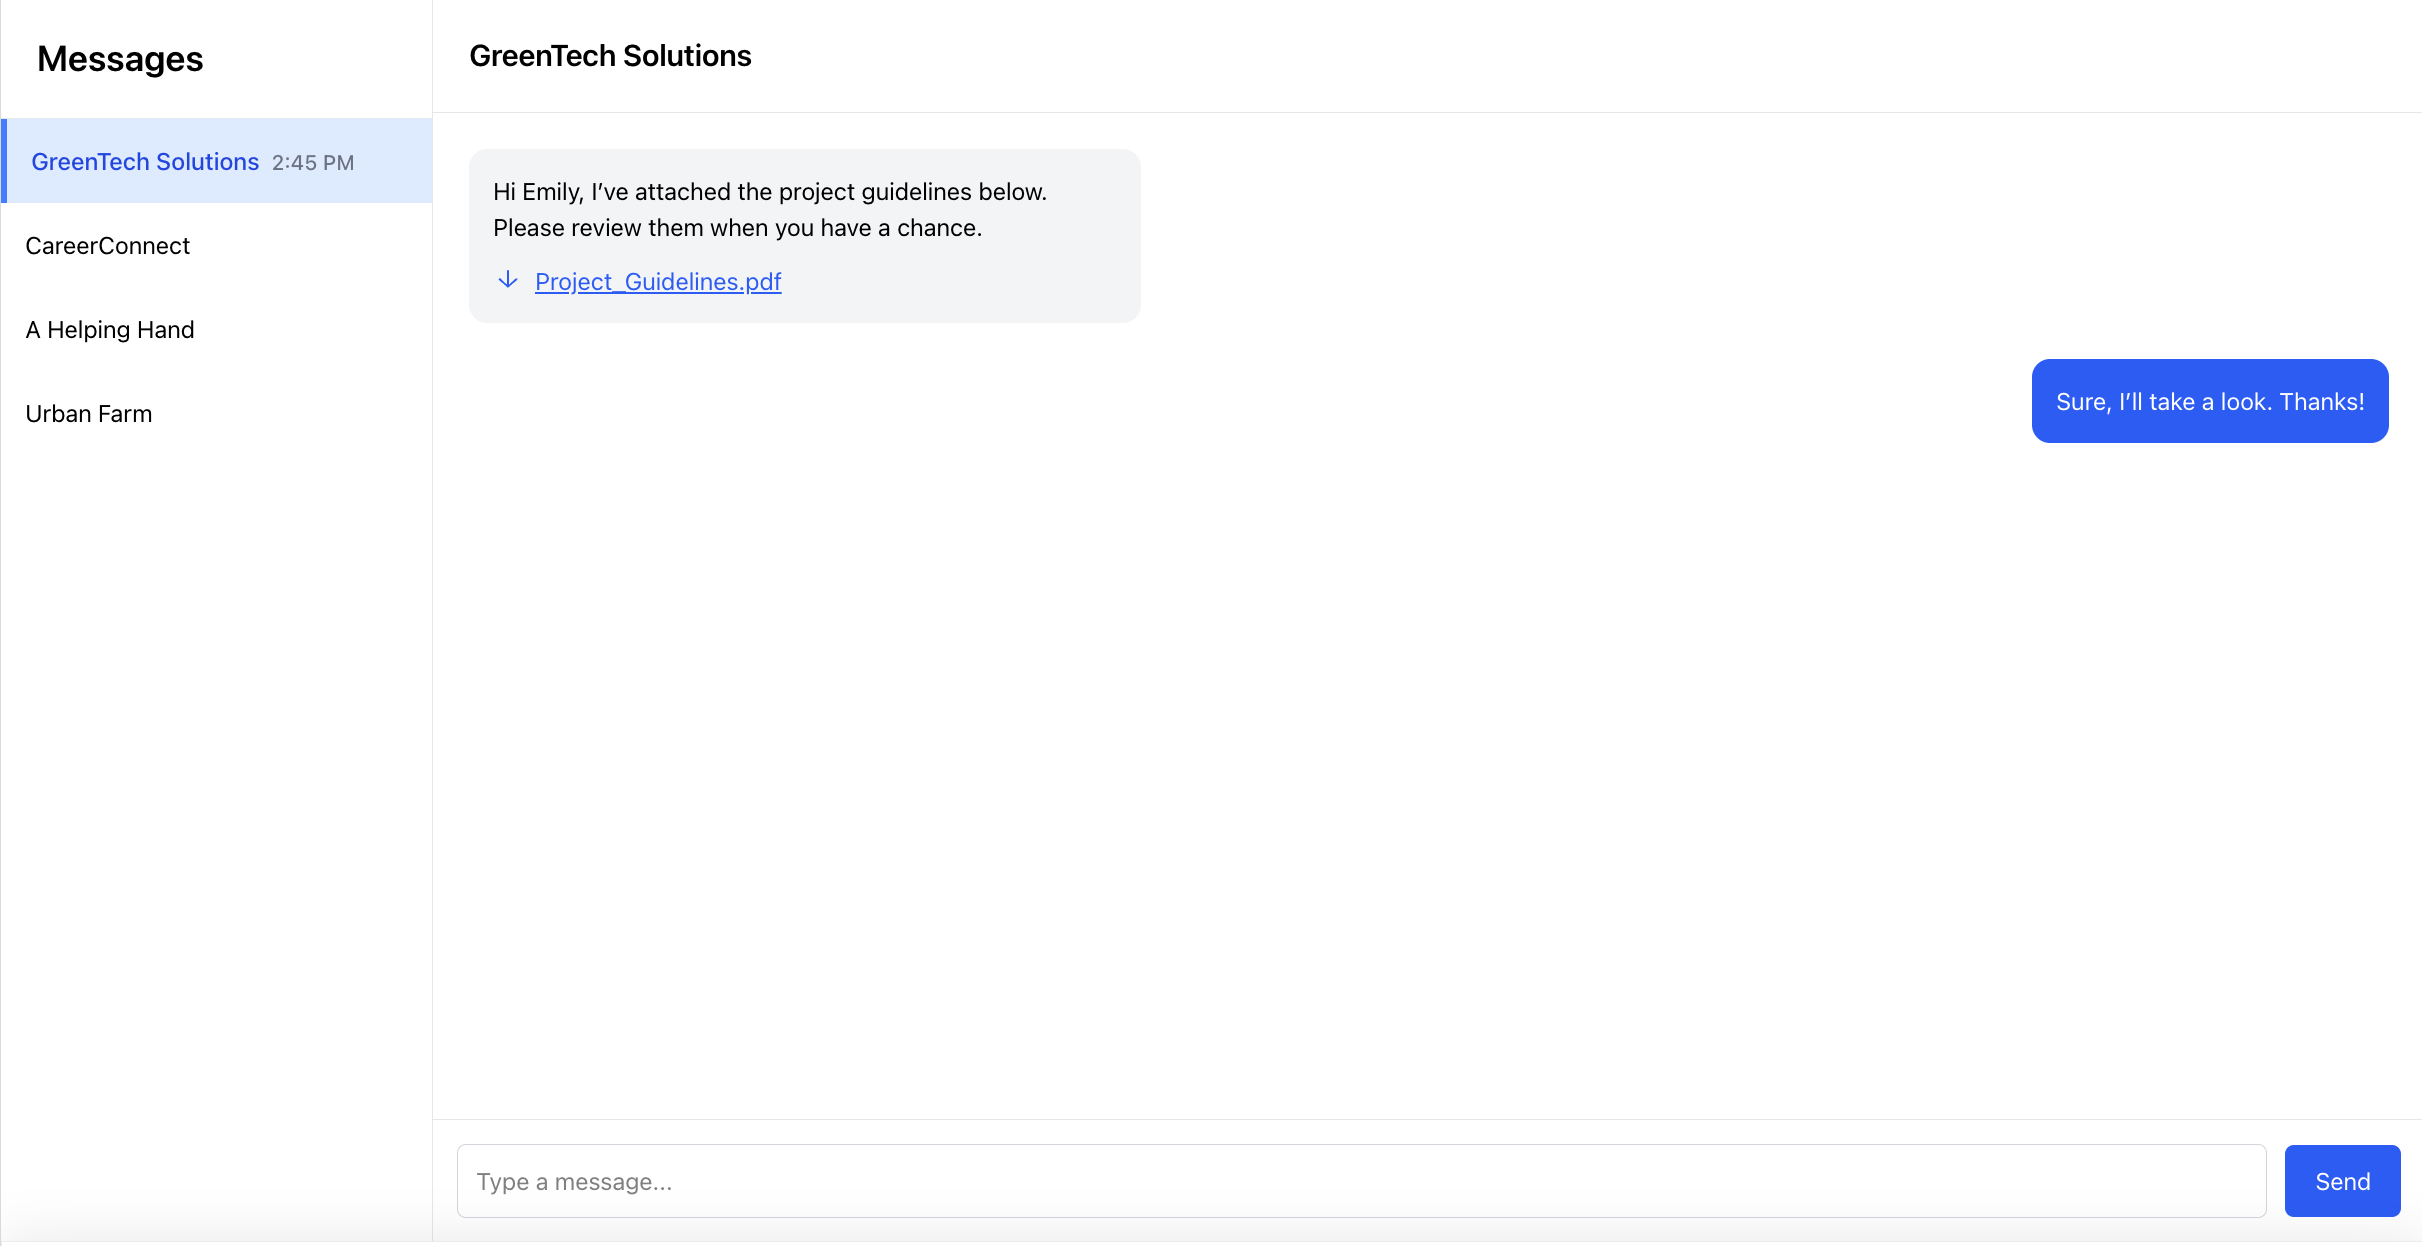
\includegraphics[width=0.85\linewidth]{figures/Messengersystem.png}
  \caption{Messaging workspace mock up coordinating inclusion support.}
  \label{fig:chat-system}
\end{figure}

To redistribute opportunities I also designed a mutual aid pool. Partners with extra capacity can offer design time, translation support, or data analysis hours. The pool uses a simple \textit{ledger system} managed by the inclusion council. Participants earn recognition badges when they contribute and can ask for help through the chat interface. Lecture 9 highlighted that platforms should support \textit{peer to peer collaboration}, and this pool puts that idea into action \citep{Lecture09}. Regular reporting on use helps keep the commitment trustworthy.
